
\section{Area Between Curves}

Recall that a definite integral calculates the signed area under a curve.  Thus, we can find the signed \integ{area between two curves} by taking their difference and integrating.  

\FormulaBox{Area Between Curves}{\begin{tabular}{c}

Let $g(x)\leq f(x)$ for all $x$ in an interval $[a,b]$. \\ Then the area bounded by the graphs \\ $x=a,$ $ x=b,$ $ y=f(x),$ and $y=g(x)$ is \\ $A=\int_a^b \left( f(x)-g(x) \right) \dif x. $
\end{tabular}}


	\begin{center}
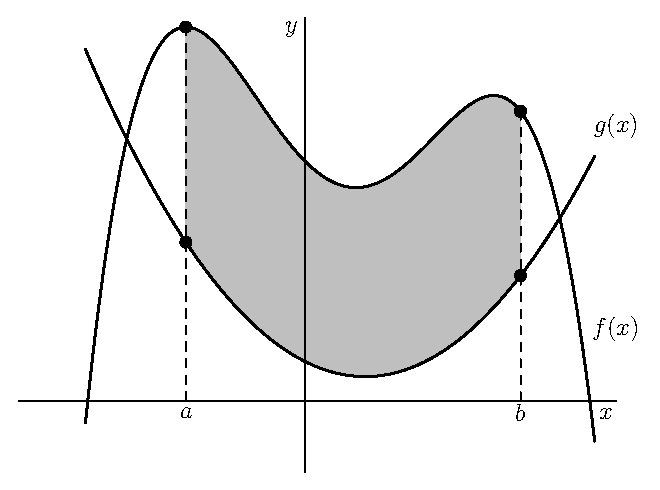
\includegraphics[width=400pt]{ChapterGeom/Figures/areabetweencurves.eps}
	\end{center}

\begin{example}{Quadrature of a Parabola}
 Suppose we wish to find the area \area{between curves} $f(x)=x$ and $g(x)=x^2$.  To accomplish this, we set the two formulas equal to each other to solve for the points of intersection.  The line and \conics{parabola} meet where  $$x^2=x \implies x^2-x=0 \implies x(x-1)=0 \implies x=0 \text{ or }  x=1.$$ 
Thus the points of intersection are at $(0,0)$ and $(1,1)$. 

	\begin{center}
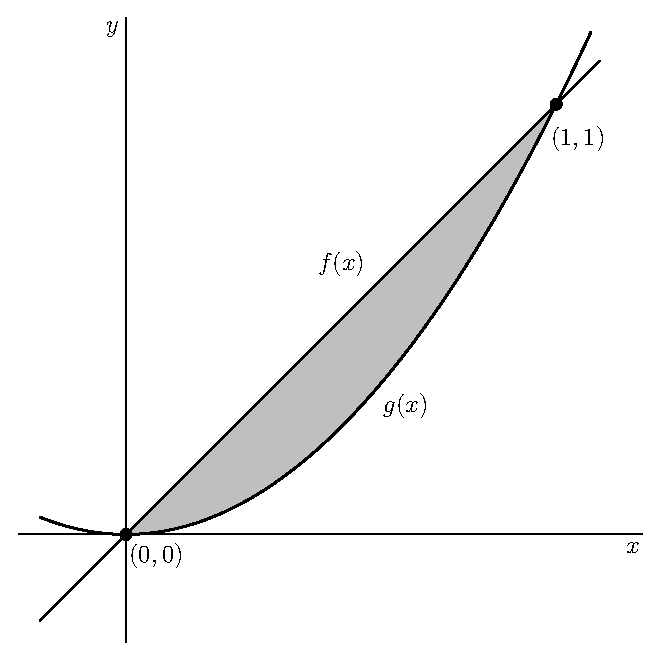
\includegraphics[width=300pt]{ChapterGeom/Figures/areabtparablin.eps}
	\end{center}
Thus, the area between curves is \begin{align*}
\int_{x=0}^{x=1}\left(x-x^2\right) \dif x &= \left. \frac{x^2}{2}-\frac{x^3}{3}\right]_{x=0}^{x=1} \\
&=\frac{1}{2}-\frac{1}{3}\\
&=\frac{1}{6}.
\end{align*}
\end{example}
\begin{comment}
\begin{exercise}{Area Between $x$ and $x^n$ \Coffeecup \Coffeecup}

For each of the listed $n\in \mathbb{N}$, take the following steps:

\begin{itemize}
\item Graph $f(x)=x$ and $g(x)=x^n$ on the same axes and shade the region bounded by the curves in the first quadrant.  Include labels of the intersection points of the curves.
\item Use an integral to find the area between curves.
\item Write the area as a decimal approximation.
\end{itemize}

Compile your results in the table below.

\begin{center}
\begin{tabular}{|c|c|c|c|} \hline
$n$ & Graph of $x$ and $x^n$ in QI & Area Between Curves in QI & Decimal Approximation \\ \hline 
& & & \\
& & & \\
3 & & & \\
& & & \\
& & & \\ \hline
& & & \\
& & & \\
4 & & & \\
& & & \\
& & & \\ \hline
& & & \\
& & & \\
5 & & & \\
& & & \\
& & & \\ \hline
& & & \\
& & & \\
6 & & & \\
& & & \\
& & & \\ \hline
& & & \\
& & & \\
7 & & & \\
& & & \\
& & & \\ \hline
& & & \\
& & & \\
8 & & & \\
& & & \\
& & & \\ \hline
& & & \\
& & & \\
9 & & & \\
& & & \\
& & & \\ \hline
& & & \\
& & & \\
10 & & & \\
& & & \\
& & & \\ \hline
\end{tabular}
\end{center}

\begin{itemize}
\item What does the area seem to be approaching as $n$ keeps getting larger?

\vspace{1in}

\item What shape does the region between the curves seem to be approaching as $n$ keeps getting larger?  Using just basic geometry, what would the area of that shape be?

\vspace{1in}

\end{itemize}

\end{exercise}

\end{comment}

Note that if the curves intersect multiple times, you might have to split the integral onto the corresponding intervals.  

\begin{example}{A Region with More Crossings}
 Find the area between the graphs of sine and cosine between $x=0$ and $x=2\pi$.

Again, to accomplish this, we set the two formulas equal to each other to solve for the points of intersection.  $$\sin(x)=\cos(x) \implies \tan(x)=1 \implies x=\pi/4  \text{ or }  x=5\pi/4$$ 
Thus the points of intersection are at $\left(\pi/4,\sqrt{2}/2\right)$ and $\left(5\pi/4,-\sqrt{2}/2\right)$. 

	\begin{center}
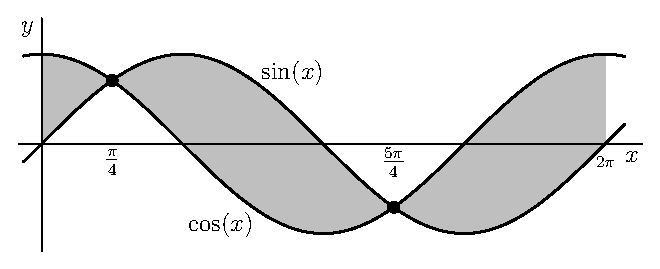
\includegraphics[width=300pt]{ChapterGeom/Figures/areabtsincos.eps}
	\end{center}

We now compute the area as follows: \begin{align*}
A&=\int_0^{\pi/4} \left(\cos(x)-\sin(x)\right) \dif x+\int_{\pi/4}^{5\pi/4} \left(\sin(x)-\cos(x)\right) \dif x+\int_{5\pi/4}^{2\pi} \left(\cos(x)-\sin(x)\right) \dif x \\
&=\left(\sin(x)+\cos(x)\right)|_0^{\pi/4} +\left(-\cos(x)-\sin(x)\right)|_{\pi/4}^{5\pi/4} +\left(\sin(x)+\cos(x)\right)|_{5\pi/4}^{2\pi}. 
\end{align*}

\end{example}
\begin{exercise}{Complete the Example \Coffeecup \Coffeecup }
Finish the computation and verify the area is 4$\sqrt{2}$.
\solushun{\begin{align*}
&\left(\sin(x)+\cos(x)\right)|_0^{\pi/4} +\left(-\cos(x)-\sin(x)\right)|_{\pi/4}^{5\pi/4} +\left(\sin(x)+\cos(x)\right)|_{5\pi/4}^{2\pi}\\
&=\left(\sin(\pi/4)+\cos(\pi/4)\right)-\left(\sin(0)+\cos(0)\right)\\
&\ \ +\left(-\cos(5\pi/4)-\sin(5\pi/4)\right)-\left(-\cos(\pi/4)-\sin(\pi/4)\right)\\
&\ \ +\left(\sin(2\pi)+\cos(2\pi)\right)-\left(\sin(5\pi/4)+\cos(5\pi/4)\right)\\
&=\left(\frac{\sqrt{2}}{2}+\frac{\sqrt{2}}{2}\right)-\left(0-1\right)\\
&\ \ +\left(-\frac{\sqrt{2}}{2}+\frac{\sqrt{2}}{2}\right)-\left(-\frac{\sqrt{2}}{2}-\frac{\sqrt{2}}{2}\right)\\
&\ \ +\left(0-1\right)-\left(-\frac{\sqrt{2}}{2}-\frac{\sqrt{2}}{2}\right)\\
&=\left(\sqrt{2}\right)-\left(1\right)\\
&\ \ +\left(\sqrt{2}\right)-\left(-\sqrt{2}\right)\\
&\ \ +\left(1\right)-\left(-\sqrt{2}\right)\\
&=4\sqrt{2}
\end{align*}
}{3in}
\end{exercise}

\begin{exercise}{A Common Mistake \Coffeecup}
 Briefly write in words, why would simply evaluating $$\int_{x=0}^{x=2\pi} \cos(x)-\sin(x) \dif x  $$ in the example above not give the area of the shaded region?

\solushun{Because the curves alternate which one is greater, the sign of the integral changes with each intersection. Thus, when $\sin(x)>\cos(x)$, the integral would be negative. So, simply summing would result in some canceling out, which would not give an accurate measure of the area between the two curves.\\}{1in}
\end{exercise}

\subsection{Area of a Circle}

Let's now prove an old friend, the formula for the \circles{area} \area{of a circle}!
\begin{exercise}{Area of a Circle \Coffeecup \Coffeecup }
\begin{itemize}
\item Recall the equation for a \conics{circle} of radius $r$ is $x^2+y^2=r^2$. Draw a diagram that shows that this equation is a consequence of the Pythagorean Theorem.  

\solushun{\\
\begin{center}
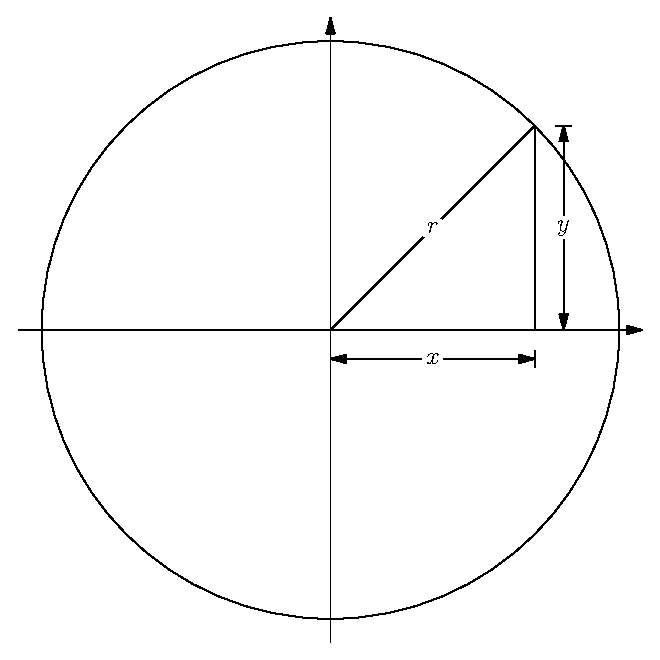
\includegraphics[width=200pt]{ChapterGeom/Figures/pythagcirc.eps}
\end{center}}{1in}

\item Solve for $y$ and note that the square root requires a ``plus or minus''.  To get the top curve $f(x)$, choose the positive square root.  To get the bottom curve $g(x)$, choose the negative square root.  Write your formulas for $f(x)$ and $g(x)$ below. \vspace*{.1in}
\begin{itemize}
\item Top Half: $f(x) = $
\vspace*{.1in}
\item Bottom Half: $g(x) = $
\vspace*{.1in}
\end{itemize}
\solushun{\vspace*{.1in}
\begin{itemize}
\item Top Half: $f(x) = \sqrt{r^2-x^2}$
\vspace*{.1in}
\item Bottom Half: $g(x) = -\sqrt{r^2-x^2}$
\vspace*{.1in}
\end{itemize}}{1in}

\item Use an integral to find the area between $f$ and $g$ to obtain the formula for the area of a circle of radius $r$.  

\solushun{\begin{align*}
\int_{-r}^{r}\sqrt{r^2-x^2}-\left(-\sqrt{r^2-x^2}\right)\dif x&=\int_{-r}^{r}2\sqrt{r^2-x^2}\dif\\
&=2\int_{-\pi/2}^{\pi/2}\sqrt{r^2-r^2\sin^2(\theta)}\cdot r\cos(\theta)\dif \theta\\
&=2\int_{-\pi/2}^{\pi/2}r^2\cos^2(\theta)\dif \theta\\
&=2r^2\int_{-\pi/2}^{\pi/2}\frac{1}{2}\left(1+\cos(2\theta)\right)\dif \theta\\
&=r^2\left[\theta+\frac{1}{2}\sin(2\theta)\right]_{-\pi/2}^{\pi/2}\\
&=r^2\left[\left(\frac{\pi}{2}+\frac{1}{2}\sin(\pi)\right)-\left(-\frac{\pi}{2}+\frac{1}{2}\sin(-\pi)\right)\right]\\
&=r^2\left[\left(\frac{\pi}{2}\right)-\left(-\frac{\pi}{2}\right)\right]\\
&=\pi r^2
\end{align*}}{2in}

\end{itemize}
\end{exercise}

\subsection{Some Other Regions for Practice}
Find the area between the following curves.  Graph the curves and shade the region! 
\begin{exercise}{Other Regions \Coffeecup \Coffeecup}

\begin{itemize}
\begin{comment}
\item $y=|x|$ and $y=\frac{1}{2}
x+1$
\vspace*{2in}

\item $y=\sqrt{x}$ and $y=\frac{1}{2}x^2$
\vspace*{2in}

\end{comment}
\item $ f(x)=x^3-x^2-x+1$ and $g(x)=x^3+x^2-x-1$
\solushun{
We start by identifying where the two graphs intersect, which we can accomplish by settings them equal and solving for $x$:
\begin{align*}
f(x)=&g(x)\\
x^3-x^2-x+1=&x^3+x^2-x-1\\
2=&2x^2\\
1=&x^2
x=\{-1,1\}
\end{align*}
So the bounds of integration are $-1,1$.
\begin{align*}
\int_{-1}^1 f(x)-g(x)\dif x&=\int_{-1}^1 x^3-x^2-x+1-(x^3+x^2-x-1)\dif x\\
&=\int_{-1}^1-2x^2+2\dif x\\
&=-2\int_{-1}^1x^2-1\dif x\\
&=-2\left[\frac{x^3}{3}-x\right]^1_{-1}\\
&=-2\left[\frac{1^3}{3}-1-\left(\frac{(-1)^3}{3}-(-1)\right)\right]\\
&=-2\left[-\frac{2}{3}-\frac{2}{3}\right]\\
&=\frac{8}{3}
\end{align*}
\begin{center}
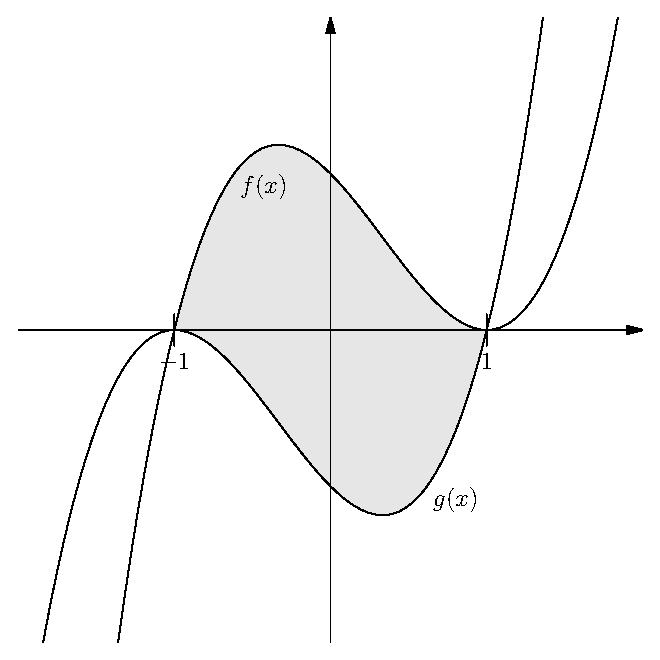
\includegraphics[width=300pt]{ChapterGeom/Figures/polyarea.eps}
\end{center}}{2in}

\item $y=\sqrt{1-x^2}$ and $y=1/2 $

\solushun{
Start by finding the bounds of integration by setting the two equations equal and finding $x$:
\begin{align*}
\sqrt{1-x^2}&=1/2\\
1-x^2&=\frac{1}{4}\\
\frac{3}{4}&=x^2\\
\pm\frac{\sqrt{3}}{2}=x
\end{align*}
Then, set up your integral, using the fact that we already found the antiderivative of a circle:
\begin{align*}
\int^{\frac{\sqrt{3}}{2}}_{-\frac{\sqrt{3}}{2}}\sqrt{1-x^2}-\frac{1}{2}\dif x&=\frac{1}{2}\left[\theta+\frac{1}{2}\sin(2\theta)\right]^{\pi/3}_{-\pi/3}-\frac{1}{2}\left[x\right]^{\sqrt{3}/2}_{-\sqrt{3}/2}\\
&=\frac{1}{2}\left[\frac{\pi}{3}+\frac{1}{2}\sin(\frac{2\pi}{3})-\left(-\frac{\pi}{3}+\frac{1}{2}\sin(-\frac{2\pi}{3})\right)\right]-\frac{1}{2}\left[\frac{\sqrt{3}}{2}-\left(-\frac{\sqrt{3}}{2}\right)\right]\\
&=\frac{1}{2}\left[\frac{\pi}{3}+\frac{1}{2}\frac{\sqrt{3}}{2}-\left(-\frac{\pi}{3}-\frac{1}{2}\frac{\sqrt{3}}{2})\right)\right]-\frac{\sqrt{3}}{2}\\
&=\frac{1}{2}\left[\frac{2\pi}{3}+\frac{\sqrt{3}}{2}\right]-\frac{\sqrt{3}}{2}\\
&=\frac{\pi}{3}-\frac{\sqrt{3}}{4}
\end{align*}
\begin{center}
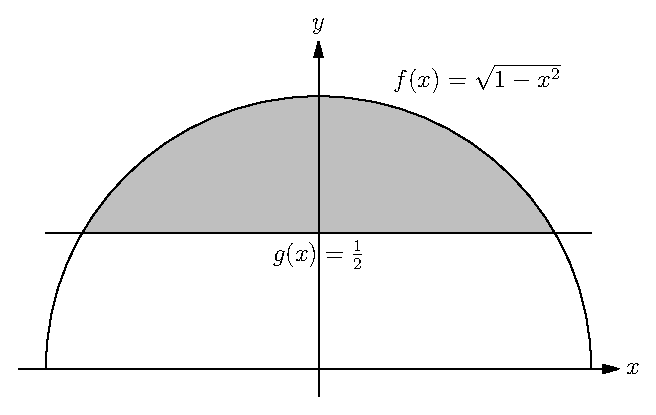
\includegraphics[width=300pt]{ChapterGeom/Figures/clippedcirc_cropped.eps}
\end{center}
}{2in}
\item $y=\tan(x)$ restricted to the domain $\left(-\pi/2,\pi/2\right)$ and $y=\frac{4}{\pi}x$

\solushun{First, find the point of intersection. A good way to do this is to graph both functions, and notice that they seem to intersect when they both equal $1$. Then, test this out by setting them both equal to 1 and solving for $x$:
$$\tan(x)=1\implies\arctan(1)=x\\
x=\frac{\pi}{4}
$$
$$\frac{4}{\pi}x=1\implies x=\frac{\pi}{4}$$
So, the functions intersect at $(\frac{\pi}{4},1)$.
A similar process produces another intersection at $(-\frac{\pi}{4},-1)$.

We need to split the integral because the functions cross at $x=0$:
$$\int_{-\pi/4}^0\tan(x)-\frac{4}{\pi}x\dif  x+\int_0^{\pi/4}\frac{4}{\pi}x-\tan(x) \dif x
$$

This gets a little messy, but since the graph is symmetrical, we can save ourselves some trouble by simply evaluating the easier integral and then doubling it.

\begin{align*}
\int_{-\pi/4}^0\tan(x)-\frac{4}{\pi}x\dif x&=\left[-\ln|\cos(x)|-\frac{2}{\pi}x^2\right]_{-\pi/4}^0\\
&=-\ln|\cos(0)|-\frac{2}{\pi}\cdot0^2-\left(-\ln\left|\cos\left(-\frac{\pi}{4}\right)\right|-\frac{2}{\pi}\left(-\frac{\pi}{4}\right)^2\right)\\
&=\ln\left|\cos\left(-\frac{\pi}{4}\right)\right|+\frac{2}{\pi}\left(-\frac{\pi}{4}\right)^2\\
&=\ln\left|\frac{\sqrt{2}}{2}\right|+\frac{2}{\pi}\left(\frac{\pi^2}{16}\right)\\
&=\ln\left|\frac{\sqrt{2}}{2}\right|+\frac{\pi}{8}
\end{align*}
So the final integral is:
$$2\left(\ln\left|\frac{\sqrt{2}}{2}\right|+\frac{\pi}{8}\right)=\left(\ln\left|\frac{1}{2}\right|+\frac{\pi}{4}\right)$$
We can simplify the logarithm a bit:
$$\left(\ln\left|\frac{1}{2}\right|+\frac{\pi}{4}\right)=\ln|1|-\ln|2|+\frac{\pi}{4}=\frac{\pi}{4}-\ln|2|$$
\begin{center}
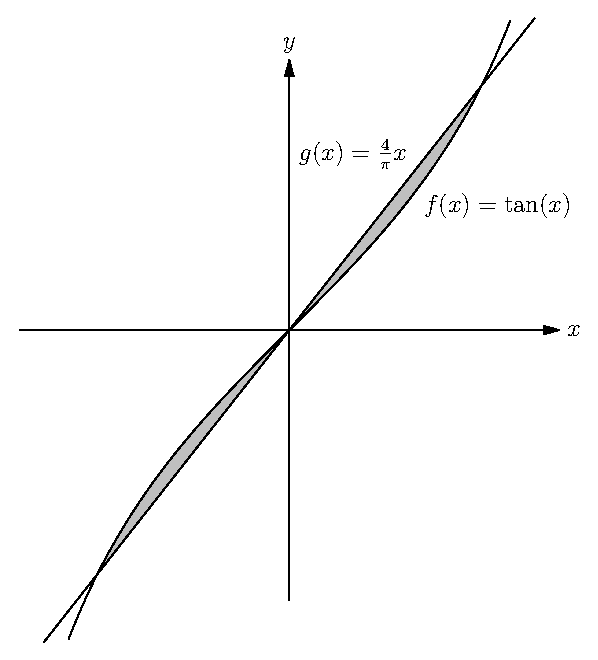
\includegraphics[width=300pt]{ChapterGeom/Figures/tangentarea.eps}
\end{center}
}{2in}

\end{itemize}
\AnswerKeyEntry{\textbullet The curves $y=x^3+x^2-x-1$ and $y=x^3-x^2-x+1$ intersect on the $x$ axis at -1 and 1 and have area 8/3 between them. 
\textbullet The area inside the unit circle but above the line $y=1/2$ is $\pi/3-\sqrt{3}/4$.
\textbullet Notice graphically that the curves intersect at $x=\pm \pi/4$.  The area between curves is $\pi/4-\ln(2)$.}
\end{exercise}
